\documentclass[11pt,a4paper]{article}
\usepackage[utf8]{inputenc}
\usepackage{amsmath}
\usepackage{amsfonts}
\usepackage{xcolor}
\usepackage{amssymb}
%\usepackage{colortbl}
\usepackage{listings}
\usepackage{hyperref}
\usepackage{graphicx}

\newcommand{\boxgreen}{\colorbox{green}{\color{black}done}}
\newcommand{\boxyellow}{\colorbox{yellow}{\color{black}in progress}}
\newcommand{\boxred}{\colorbox{red}{\color{black}NYI}}

% Counter for the requirements
\newcounter{reqc} 
\newcommand{\reqID} {%
   \stepcounter{reqc}%
   \thereqc}

% Counter for the figures/images
\newcounter{figc}
\newcommand{\figID} {%
   \stepcounter{figc}%
   \thefigc}
   
% Counter for the tables
   \newcounter{tabc}
\newcommand{\tabID} {%
   \stepcounter{tabc}%
   \thetabc}


\author{David Sverdlov \\ dsverdlo@vub.ac.be}
\title{Bachelorproef AMuRate: Voortgangsrapport\\ 3e Bachelor Computerwetenschappen}
\begin{document}
% Begin title page
\begin{flushleft}
\noindent 
\includegraphics[width=0.6\linewidth]{vub_logo.jpg} 
\end{flushleft}
{\let\newpage\relax\maketitle} % don't let it set newpage

\begin{center}

\includegraphics[width=4cm]{amr_gold_thick.png} 
\end{center}



\newpage
\tableofcontents

\newpage
\section{Inleiding}
	\subsection{Doel}
De uitdaging van dit bachelorproject is om een applicatie te ontwikkelen voor het mobiele platform Android. De applicatie moet gebruikers in staat stellen om muzieknummers op te zoeken en een beoordeling te kunnen geven. Die scores worden dan opgestuurd naar een data-collection server met een database, waar later recommendeer algoritmen op zullen werken. (De implementatie daarvan valt niet binnen de scope van dit project.) \\
Dit project wordt gepromote door prof. Dr. Ann Nowé en begeleidt door Maarten Deville en Peter Vranckx. 

	\subsection{Referenties}
		\subsubsection{AMuRate homepagina}
			\url{http://dsverdlo.github.com/AMuRate}
		\subsubsection{Android}
			\url{http://www.android.com/}
		\subsubsection{Ice Cream Sandwich}
			\url{http://www.android.com/about/ice-cream-sandwich/}	
		\subsubsection{Last.fm}
			\url{http://www.last.fm/home}	
		\subsubsection{Github}
			\url{https://github.com/}

	\subsection{Afkortingen en definities}
		\subsubsection{API}
		API staat voor Application Programming Interface en zorgt voor de communicatie tussen programmas, door de scheiding te vormen tussen verschillende lagen van abstracties.
		\subsubsection{XML/JSON}
		XML staat voor Extensible Markup Language en is een van de meest gebruikte opmaaktalen, die gestructureerde gegevens kunnen omzetten in platte tekst. (Om het zo makkelijk(er) door te kunnen sturen.)
		\newline
		JSON is aan afkorting van JavaScript Object Notation en is een alternatieve simpele manier om objecten voor te stellen als platte tekst.
		\subsubsection{HTTP}
		HTTP staat voor HyperText Transfer Protocol en is het medium tussen een webbrowser en een webserver. Die communicatie gebeurt door middel van URLs, die verwijzen naar 'iets' op een of andere webserver.
		\subsubsection{GUI}
		GUI staat voor Graphical User Interface en is een visuele vormgeving van een programma, dat door middel van knoppen, afbeeldingen, ... gebruikers toelaat om op een gebruiksvriendelijkere manier met de applicatie om te gaan .

\section{Achtergrond}
	\subsection{Last.fm/api: REST}
Om informatie (over muziek in dit geval) op te kunnen zoeken, moet er gebruik gemaakt worden van een online database met een openbare en hanteerbare API. \textit{Last.fm} is een muziek recommendation service met een enorme online muziek database, die  een gratis (lees: voor geregistreerde gebruikers) API aanbiedt, die iedereen toelaat om mobiele/desktop programmas of web services te bouwen met hun data.
\newline
Die procedure verloopt als volgt: om data uit de database te halen moet er een call (oproep) gestuurd worden. Deze gebeurt via HTTP GET naar de Last.fm server die op zijn beurt antwoordt met een XML object (of JSON op aanvraag). De methode van operatie die hier gebruikt wordt heet 'REST'. 
	\subsection{REST architectuur}
	REST staat voor Representational State Transfer en is een type van architectuur voor bepaalde gedistribueerde systemen (zoals het World Wide Web), waarin een duidelijke onderscheiding wordt gemaakt tussen client en server. Clienten kunnen oproepen doen naar de server, die de oproepen analyseert, een antwoord formuleert, en dat antwoord terug naar de klant stuurt. REST maakt gebruik van werkwoorden en zelfstandige naamwoorden om de oproepen ook leesbaar voor mensen te maken. De standaard werkwoorden zijn GET, POST, PUT en DELETE, om data te kunnen verkrijgen, wijzigen of opsturen.
	
\section{Voorgrond}
	\subsection{Website}
		In dit project wordt er gebruik gemaakt van Git als versiebeheersysteem, omdat het een gratis, eenvoudige en betrouwbare manier is om de broncode te beheren. Om updates in het project naar de repository te sturen wordt er gebruikt gemaakt van Github voor Windows. Nog een voordeel van deze keuze is dat Github de mogelijkheid biedt om snel en simpel websites te maken(en te behoren) voor de bestaande projecten. Zo werd er een kleine website voor dit project opgesteld, die terug te vinden is op: \url{http://dsverdlo.github.com/AMuRate/}. Hier kan men de open-source broncode bekijken, het logboek of dit document raadplegen, en de applicatie (.apk) downloaden voor Android 4.0 toestellen.
	\subsection{Naam en logo}
		De naam van een project geeft meestal een kleine beschrijving van wat de applicatie doet/ waar hij voor dient. AMuRate komt van "Android Music Rating". Omdat het project vooral geïmplementeerd zou worden via een Android emulator, en simpelweg "AMR" te kort en onduidelijk zou zijn, werd er gekozen voor AMuRate. Het logo (zoals te zien op de voorpagina) is een compositie van een 5-ster in een bol die iets weg heeft van een "dragon ball" (uit de Japanse animatieserie DragonBall Z). In DBZ bestaan er maar 7 bollen op de hele wereld en wanneer die allemaal verzameld zijn, mag de beheerder een wens doen. Een beetje gelijkaardig aan hoe elke artiest hoopt 5 sterren (/ 7 dragon balls) te verzamelen. 
	In de ster zelf zijn drie letters gekleurd ("AMR"), naar de naam van de applicatie.
	
\section{Vereisten}
	% Get a nice table with colors running here, bro
	\begin{tabular}{| l | l | c | r |}
	\hline
	ID 		& 	Priority	&	Beschrijving						& Status \\ \hline \hline
	\reqID	&	necessity	&	Titel (en artiest) opzoeken			& \boxgreen \\ \hline
	\reqID 	& 	necessity	&	Track weergeven						& \boxgreen \\ \hline
	\reqID	& 	necessity	&	Enkel op artiest opzoeken 			& \boxyellow \\ \hline
	\reqID 	& 	optional	&	Album tonen 						& \boxgreen \\ \hline
	\reqID	& 	necessity	&	Score opslagen in database 			& \boxgreen  \\ \hline
	\reqID 	& 	necessity	&	Score ophalen in lokale database 	& \boxgreen \\ \hline
	\reqID	& 	necessity	&	Score opsturen naar remote db		& \boxred \\ \hline
	\reqID	& 	optional	&	Zoek geschiedenis opslagen			& \boxyellow \\ \hline
	\reqID	&	optional	&	Stream$/$preview 30sec songs		& \boxyellow \\ \hline
	\reqID	&	optional	&	Caching implementeren				& \boxred \\ \hline
	\reqID 	& 	optional	&	Onderzoek uitbreidbaarheid (ios?)	& \boxred \\ \hline
	\reqID 	&	optional	&	Informatie ophalen van media speler & \boxred \\ \hline
	
	\hline	
	\end{tabular} \\ \newline
	\small \textit{Tabel \tabID : Vereisten van het project met uitleg en implementatiestatus.} \normalsize
	
\section{GUI}
	Hieronder volgen enkele schermopnames van de voorlopige GUI. Deze zal normaal gezien niet veel meer veranderen naar het verloop van de rest van het project, maar men kan nooit zeker weten.\\
	Voor het voorbeeld toon ik eerst het startscherm waar men mee begint wanneer de applicatie gestart wordt. Men kan kiezen
	
	\begin{tabular}{l l l}
	
	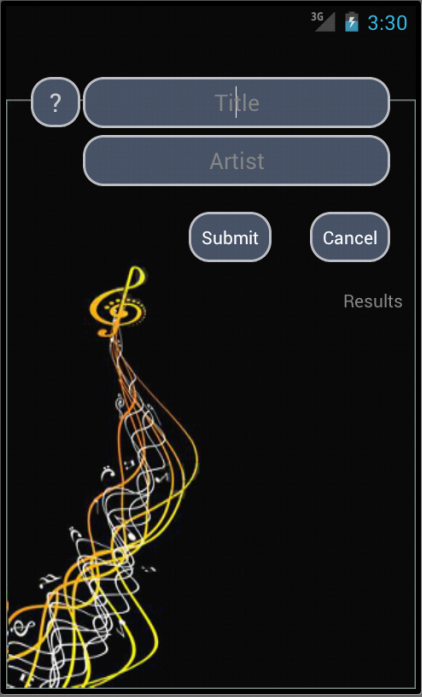
\includegraphics[scale=0.4]{GUI_0124_startscreen.png} &	
	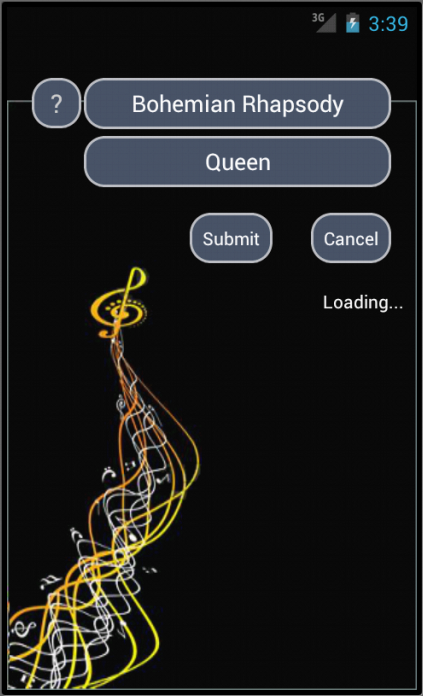
\includegraphics[scale=0.4]{GUI_0124_startsearch.png} &
	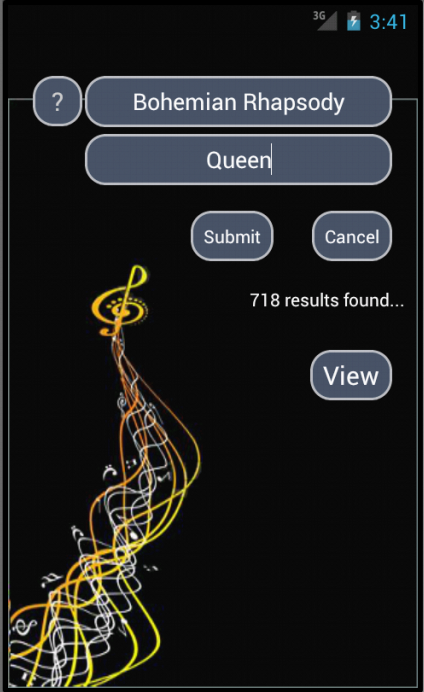
\includegraphics[scale=0.4]{GUI_0124_startresults.png} \\
	
	Start scherm & Zoek- en downloadproces & Klaar met downloaden \\[5ex]
	
	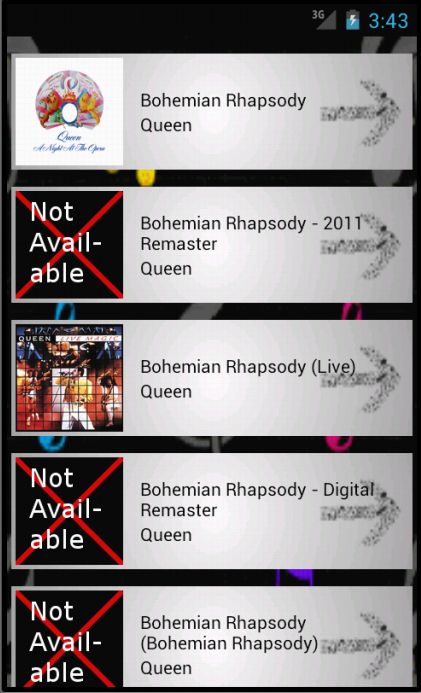
\includegraphics[scale=0.4]{GUI_0124_results.png} &
	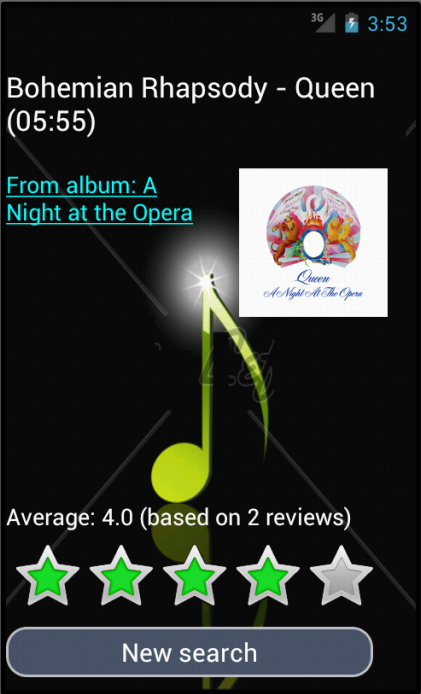
\includegraphics[scale=0.4]{GUI_0124_track.png} &
	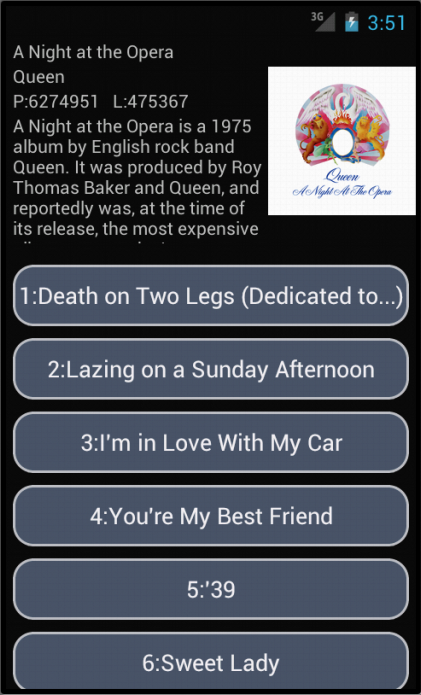
\includegraphics[scale=0.4]{GUI_0124_album.png} \\
	Geeft alle resultaten weer & Weergave van een track & Albumscherm \\
	
	\end{tabular}
	
\section{Implementatie}
	\subsection{Packet onderverdeling}
		\normalsize De broncode van het project is opgedeeld in 3 packets: \textit{gui, objects en services}. In het \textit{GUI} packet zitten alle activities\footnote{Dit is de naam van een scherm in Android}. Elk scherm heeft een aparte activity nodig. \\
		In het \textit{objects} packet zitten de objecten, die abstractie brengen in het project. Bijvoorbeeld wanneer een track opgezocht werd en klaar is met downloaden, zal het omgezet worden in een klasse Track. Zo moet de GUI zich niets aantrekken van hoe de representatie eruit zag toen het van de server kwam. \\
		Packet \textit{services} bevat de klassen die instaan voor verschillende diensten die moeten gebeuren in het project. Zo is er de MyConnection klasse, die de oproepen doet en antwoorden download van de Last.fm API. De database beheerder klasse is ook een dienst die verleend wordt aan het project, en bijgevolg ook in dit packet zit.
	\subsection{Database}
	\subsubsection{Lokale Database}
	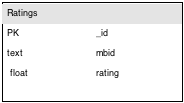
\includegraphics[scale=1]{DatabaseScheme.png} \\
	\small \textit{Afbeelding \figID : Dit schema stelt het model voor van de database.} \\ \normalsize
	
De lokale database moet data bijhouden die offline geraadpleegd zou willen worden. Hierbij reken ik op een geschiedenis van de laatste zoekopdrachten en van de laatst gegeven scores. Aangezien deze applicatie vooral beroep doet op een actieve internetverbinding, zal er niet veel meer dan dat opgeslagen worden. \\
	 De implementatie van deze database gebeurt via SQLite.
	\subsubsection{Externe Database}
	Het design van de externe database zal ontworpen moeten worden met oog op de recommender algoritmen, die er later op 'losgelaten' gaan worden. Hier zal later meer informatie over komen.
		
\section{Voortgang}
Voor ik de voortgang van dit project begin te bespreken, eerst een klein overzicht van de hoogtepunten in het project tot nu toe. \\

	\begin{tabular}{| c | p{\linewidth} | }
	\hline
	Datum & Informatie \\ \hline \hline 
	24-10 & Informatie ontvangen i.v.m. opdracht \\ \hline
	07-11 & Afspraak met begeleiders en promoter, acceptatie bachelorproef \\ \hline
	21-11 & Android project aangemaakt met simpele GUI. Ook Last.fm account aangemaakt en unieke API sleutel aangevraagd. \\ \hline
	05-12 & Gebruikers kunnen echte calls maken en muziek opzoeken. Zitten nog bugs in en er kan nog niet gezocht worden naar artiesten \\ \hline
	19-12 & Er kan ook gezocht worden op artiesten, GUI werd herzien, abstractie in code toegevoegd. \\ \hline
	03-01 & Een score kan worden opgeslagen in de lokale database, en het totaal en gemiddelde kan uitgelezen worden. \\ \hline
	xx-xx & Todo: Titel en artiest opslagen voor geschiedenis GUI. Ook nog op artiest kunnen zoeken. Caching implementeren. Ook alle bugs eruit halen. \\ \hline
	
	\end{tabular} \\ 
	\small \textit{Tabel \tabID : Enkele belangrijke highlights in de voortgang van het project.} \newline \normalsize
	

Zoals in de sectie Vereisten gezien kan worden (met bewijs van sectie GUI), is de applicatie langs de client-kant bijna volledig af. Men kan al muziek nummers opzoeken, selecteren en beoordelingen geven die effectievelijk opgeslagen worden. Wat er aan deze kant nog ontbreekt is een manier om enkel op artiest te zoeken, geschiedenis te kunnen bekijken, en eventueel als er nog tijd is: caching implementeren om het verbruik en duratie van de internetverbinding op een minimum te houden. \\
Deze dingen staan vanboven op de TODO lijst. Daarna zal er aan de serverside gewerkt worden. Eens de werking van de recommendeer algoritmen beter bekend is, kan de externe database hiernaar opgezet worden, en moet er een aangepaste synchronisatie gebeuren tussen de twee databases.
	
\section{Bronnen / Tools}

\subsection{Eclipse}
Programmeerplatform Eclipse (Juno) werd gebruikt voor de implementatie en emulatie.	\\
\url{http://www.eclipse.org/}

\subsection{Android Development Toolkit (ADT)}
Deze plug-in bevat alle benodigdheden om programma's voor Android in Eclipse te bouwen en testen.\\
\url{http://developer.android.com/sdk/index.html}

\subsection{Verschillende informatie}
En voor alle vragen klein tot groot op te lossen, rare errors/bugs te vinden of een diepere verstanding te krijgen van bepaalde termen:\\
\url{https://www.google.be/} \\
\url{http://www.wikipedia.org/} \\
\url{http://stackoverflow.com/}
\end{document}